%!TEX program= xelatex
\documentclass[oneside,table]{ntuthesis}
\usepackage{enumerate}
\usepackage{times}
\usepackage{wallpaper}
\usepackage{verbatim}
\usepackage{color}
\usepackage{url}
\usepackage{graphicx,dcolumn,bm}
\usepackage{graphicx}
\usepackage{array}
\usepackage{subfigure}
\usepackage{amsfonts}
\usepackage{amsmath}
\usepackage{amssymb}
\usepackage{array,booktabs,arydshln,xcolor}
\usepackage{indentfirst}
\usepackage{pdfpages}
\usepackage{multirow}
\usepackage{caption}
\usepackage{xcolor}
\usepackage[sort&compress,numbers]{natbib}
%\usepackage{doi}%<----------
\usepackage{nicefrac}
\usepackage[section]{placeins}

\newcommand\VRule[1][\arrayrulewidth]{\vrule width #1}
\newcommand{\Hamiltonian}{\mathcal{H}}
\newcommand{\rb}{\right}
\newcommand{\lb}{\left}
\newcommand{\nearint}{\sum_{\lb<i,j \rb >}}
\newcolumntype{L}[1]{>{\raggedright\let\newline\\\arraybackslash\hspace{0pt}}m{#1}}
\newcolumntype{C}[1]{>{\centering\let\newline\\\arraybackslash\hspace{0pt}}m{#1}}
\newcolumntype{R}[1]{>{\raggedleft\let\newline\\\arraybackslash\hspace{0pt}}m{#1}}
\definecolor{llblue}{rgb}{0.9000,0.9,1.0}
\DeclareMathOperator{\Tr}{Tr}

% uncomment this if you want to indent the first paragraph
\usepackage{indentfirst}

% uncomment this if you want to make pdf file with hyperlink
\usepackage[colorlinks=false]{hyperref}

% \CenterWallPaper{0.174}{watermark.pdf}
% \setlength{\wpXoffset}{6.1725cm}
% \setlength{\wpYoffset}{10.5225cm}

\makeatletter
\g@addto@macro\normalsize{%
  \setlength\abovedisplayskip{8pt}
  \setlength\belowdisplayskip{8pt}
  \setlength\abovedisplayshortskip{8pt}
  \setlength\belowdisplayshortskip{8pt}
  \setlength{\parskip}{8pt}
}
\makeatother
\hypersetup{
	pdfauthor={Wu, Po-Kuan},
	pdftitle={Classical Monte Carlo Studies on 3D XY Models with Effects of Nonlinearity and Anisotropy},
	pdfsubject={Master Thesis}
}


% Using the tex-text mapping for ligatures etc.
\defaultfontfeatures{Mapping=tex-text}

% Set the default fonts
\setmainfont{Times New Roman}
\setCJKmainfont[AutoFakeBold=2,AutoFakeSlant=.4]{DFKai-SB}



% Your information goes here
% author: Tz-Huan Huang [http://www.csie.ntu.edu.tw/~tzhuan]

% ----------------------------------------------------------------------------
% "THE CHOCOLATE-WARE LICENSE":
% Tz-Huan Huang wrote this file. As long as you retain this notice you
% can do whatever you want with this stuff. If we meet some day, and you think
% this stuff is worth it, you can buy me a chocolate in return Tz-Huan Huang
% ----------------------------------------------------------------------------

% Syntax: \var{English}{Chinese}
\university{National Taiwan University}{國立台灣大學}
\collage{College of Science}{理學院}
\institute{Department of Physics}{物理學系}
\title{Comparison between Tensor Network Algorithms for Two Dimensional Infinite Quantum Many-Body Systems}{比較不同張量網路演算法應用在二微多體量子物理系統之優劣}
\author{Yun-Hsuan Chou}{周昀萱}
\studentid{R02222062}
\advisor{Ying-Jer Kao, Ph.D.}{高英哲 博士}
\year{2016}{105}
\month{April}{4}
\day{3}


\begin{document}

\frontmatter

\makecover

%\makecertification
 \newpage
 \thispagestyle{empty}
 \mbox{}
%\includepdf[pages={1}, pagecommand={}]{plots/output.pdf}

\begin{acknowledgementszh}
隨著時光流逝,終於完成了我在物理系的碩班生涯。比起大學在材料系的無聊日子,這三年的經歷讓我感到彌足珍貴。

首先我要感謝高英哲老師的指導與包容。讓比較晚才理解並進入狀況的我也能有機會學習現在十分流行的 Tensor Network 演算法並參與開發 Uni10 的工作,讓我了解在設計CPU與GPU程式時該有的相關資訊與技巧。並在我研究十分掙扎時給予我研究的方向與建議,也讓我有許多機會與其他學者討論以克服問題,對於我的研究有了長足的幫助。

再來是要感謝組上的同學。其中特別感謝謝昀達學長在他繁忙日程裡,仍撥隴指導一個剛開始不怎麼會寫 c/c++ 的菜鳥,並讓我對 Tensor Network 相關的演算法有更進一步的認識。再來我想感謝從未謀面的張學文學長,許許多多研究上的問題,都可以在神秘的玩貝資料夾中得到答案或起發。還要感謝感謝楊淵棨學長、吳柏寬學長、郭子傑學長、李致遠學長、高文瀚、林育平、易德、吳凱析對於我研究與課業上的種種幫助。其中特別感謝吳柏寬學長與林育平,除了對於我在物理理論、學業和娛樂上的幫忙外,也讓本應因研究卡關而在研究室崩潰的夜晚變得十分熱鬧充滿活力,並授與了我二階張亮黑魔導的頭銜。

最後,十分想感謝我的父母。不論我的選擇結果是好與壞、風險高或低,總是不斷地給與我精神上的鼓勵與物質上的支持,感謝你們的包容,才我能讓我毫無顧慮、充實的過完我碩班的時光,體驗著不一樣的人生。
\end{acknowledgementszh}

%\begin{acknowledgementsen}
%I'm glad to thank\ldots 
%\end{acknowledgementsen}

%!TEX root = thesis.tex
\begin{abstractzh}
如何判斷多體量子系統的相變化,在
\end{abstractzh}

\begin{abstracten}
In statistical and condensed matter physics, the phase transition and the critical behavior are very important topics.
\end{abstracten}

\begin{comment}
\category{I2.10}{Computing Methodologies}{Artificial Intelligence --
Vision and Scene Understanding} \category{H5.3}{Information
Systems}{Information Interfaces and Presentation (HCI) -- Web-based
Interaction.}

\terms{Design, Human factors, Performance.}

\keywords{matrix product state(MPS), projected entangled pair state(PEPS), projected entangled simplex state, infinite time-evolveing block-decimation, corner transfer matrix, tensor renormalization group, lBenchmarks, uni10.}
\end{comment}


\tableofcontents
\listoffigures
\listoftables

\mainmatter

% Your thesis goes here
%!TEX root = thesis.tex
\chapter{Introduction}
\label{chapter:Introduction}

\section{Overview}
\label{overview}
	bond dimension is too big to do simulation.



\svnInfo $Id: state.tex 22814 2011-12-20 15:00:19Z kohlhase $
\svnKeyword $HeadURL: https://svn.kwarc.info/repos/kwarc/doc/macros/forCTAN/proposal/dfg/examples/proposal/state.tex $

\section{State of the Art and Preliminary Work \deu{(Stand der Forschung und eigene Vorarbeiten)}}\label{stand}

\subsection{List of Project-Related Publications \deu{(Projektbezogenes Publikationsverzeichnis)}}

\begin{todo}{from the proposal template}
  Please include a list of own publications that are related to the proposed project. It
  serves as an important basis for assessing your proposal. The number of publications to
  cite here is determined as follows:
  \begin{compactdesc}
    \item[Single applicant] two publications per year of the funding duration
    \item[Multiple applicants] three publications per year of the funding duration
    \end{compactdesc}
    These rules refer to the proposed funding duration for new proposals and the completed
    duration for renewal proposals.
    
    If you are submitting a proposal to the DFG for the first time and have therefore not
    published in the proposed research area, please list the up to five most important
    publications so far.
\end{todo}

\subsubsection{Peer-Reviewed Articles \deu{(Artikel mit wissenschaftlicher Qualitätssicherung)}}

\dfgprojpapers{Kohlhase:pdpl10,providemore}

\ednote{Anmerkung Jens: Ein nützliches Feature wäre hier, wenn das Paket eine (eventuell
  über Optionen der Dokumentklasse unterdrückbare) Warnung ausgeben würde, wenn zu viele
  Publikationen entsprechend DFG-Richtlinien angegeben werden. Die Anzahl ist sehr eng
  begrenzt.}

\subsubsection{Other Articles \deu{(Andere Artikel)}} None.

\subsubsection{Patents \deu{(Patente)}} None.

%%% Local Variables: 
%%% mode: LaTeX
%%% TeX-master: "proposal"
%%% End: 

% LocalWords:  subsubsections dfgprojpapers pdpl10 providemore compactdesc
% LocalWords:  ourpubs nociteprolist KohKoh ccbssmt09 KohRabZho tmlmrsca10
% LocalWords:  Hutter09 sifemp09

%!TEX root = thesis.tex
\chapter{2-D Imaginary Time Evolving Block Decimation}
\label{chapter:2ditebd}

In this chapter we introduce some different ways to implement two-dimensional imaginary time-evolving block decimation and apply them in calculation of ground state of Heisenberg and transverse Ising model on two-dimensional square lattice. In section \ref{ite} and \ref{itebd}, we briefly review the idea of imaginary time evolution (iTEBD),[\ref{vidal}] and explain how to extend it to two-dimensional [\ref{X,zhon}]. Second, we briefly review another method to make 2D-iTEBD more stable[\ref{1.1}]. In the last section \ref{2dopt}, we record various particulars which are helpful optimizing algorithms.

\section{Imaginary Time Evolution}
\label{ite}
Theoretically, if having the imaginary time evolution operator $e^{-\tau H}$, we could project any random states to the ground state, as long as the wave-function can be written as,
\begin{align}
	\label{mapgroud}
	\Ket{\psi_0} = \frac{e^{\tau H} \Ket{\Psi}}{\parallel e^{\tau H} \Ket{\Psi}\parallel}
\end{align}
but according to the eq.\ref{mapgroud}, we may found that the number of coefficients in an origin evolution operator $e^{-\tau H}$ is proportional to $2^N \times 2^N$. On the other words, it is impossible to update entire system directly. In order to restricting the rapid dimensional growth, we apply \textit{Suzuki Trotter decomposition}[\ref{1.1}][\ref{1.1}] to approximate. The main idea of \textit{Suzuki Trotter} is decomposing the whole system to lots of units cell and using some smaller operations to update the wave-function.
\begin{align}
	\label{STd}
	e^{\delta A + B} = e^{\delta A}e^{\delta B} + O(\delta^2)
\end{align}
eq.\ref{STd} means the first-order Suzuki Trotter  decomposition, and A and B are non-commutative with each other.

Now that the dimension of the evolution operator is reduced to a n-site operator and in chapter \ref{chapter:properties}, we have shown that a many-body system can map to a MPS or PEPS structure, so we can draw the process of updating a ground state like Fig.\ref{fig312},

\begin{figure}[ht]
	\centering
	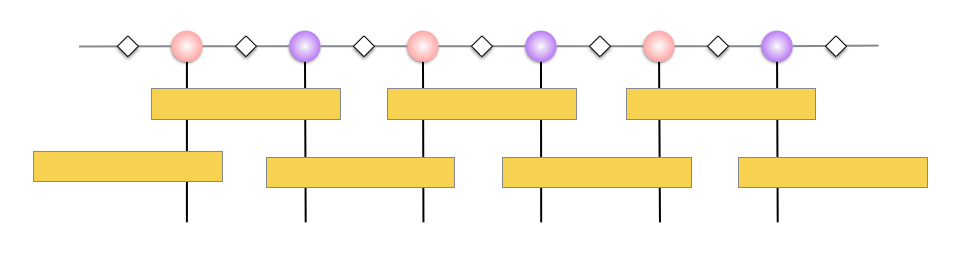
\includegraphics[width=0.75\textwidth]{figures/fig312.png}
	\caption[The picture of the main idea of itebd.]{The red and blue tensor denotes on \textit{odd} and \textit{even} sites. The yellow one are time evolution operators $e^{-\tau H_{k,k+1}}$, $e^{-\tau H_{k+1,k}}$}
	\label{fig312}
\end{figure}

On the other work, contract the tensors in Fig.\ref{fig312} repeatedly until the ground state energy to the minimum. The remained tensor is considered as the ground state of the system. So the next question: How can we contract them and preserve the structure like Fig{\ref{fig311}}? This answer is iTEBD.

\begin{figure}[ht]
	\centering
	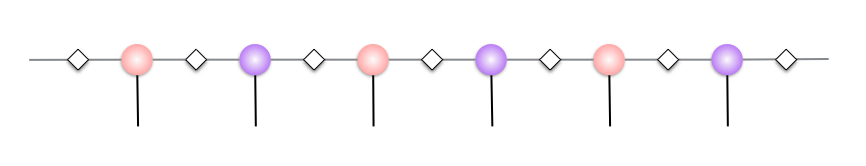
\includegraphics[width=0.75\textwidth]{figures/fig311.png}
	\caption[The picture of matrix product states]{The simple form of a matrix product state.}
	\label{fig311}
\end{figure}

\section{Simple Infinite Imaginary-Time Evolving Block Decimation for 2-D system}
In this section, we apply the TN diagrams to introduce the methods of implementation of algorithm. If you are interested in the mathematical formula of them, please read the references \citep{vidal_efficient_2004} [\ref{dd}][\ref{eaef}], witch include more details of theoretical discussion.

\label{itebd}
\subsection{Simple Description of iTEBD for 1-D system}

The algorithm start from 2 random states and 2 random diagonal matrices which are considered as entanglement between particles. In the TN diagrams, Fig.\ref{fig313}, the states and entanglement between neighbor sites are represented by the nodes and bonds with different colors.

\label{1ditebd}
\begin{figure}[ht]
	\centering
	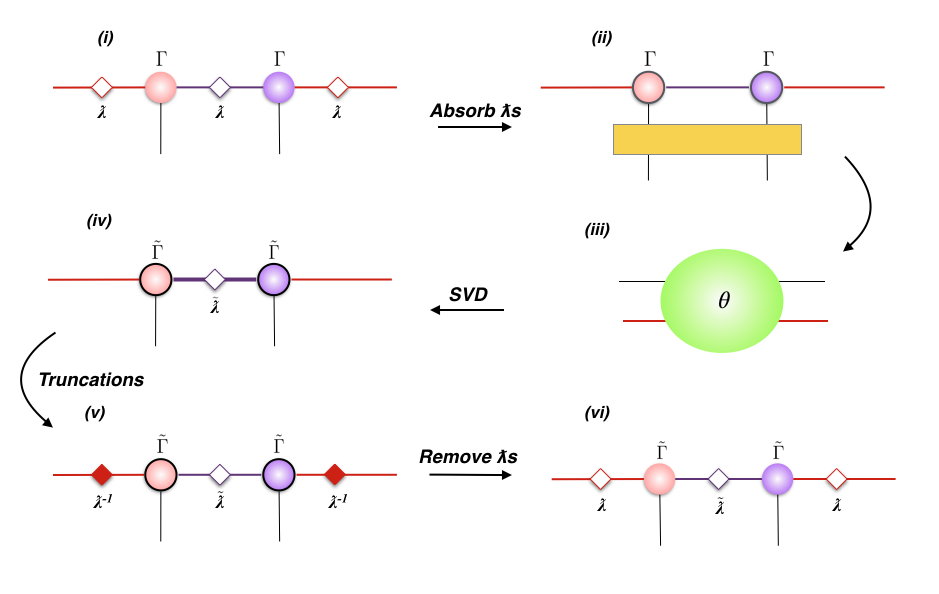
\includegraphics[width=0.90\textwidth]{figures/fig313.png}
	\caption[The tensor network diagrams for the 1-D iTEBD]{ (i)Absorb all $\lambda$ to $\Gamma$. (ii) Contract an evolution operator $e^{-\delta H}$ for evolving the system. (iii) Decompose the tensor $\theta$ by SVD. (iv) Truncate and Update the states and $\lambda$ on the green bond.(v) Remove $
		\lambda$ for obtaining the states. (iv) After updating the states and $\lambda$ on the purple bond, apply the way to update the red bond and repeat all the steps until the ground state convergence.}
	\label{fig313}
\end{figure}

The processes shown in Fig.\ref{fig313} is a standard strategy for implementation of iTEBD and also called \textit{Simple Update}. 

In one dimensional system, the performance of Simple Update is pretty well, because 1-D systems obey the canonical form and have less influences of environment. However, in 2-D systems, due to the area law, we need consider the environment more restrictively when measuring the local observable. Moreover, the computational consumption is another serious problem, owing to the growth of a state's dimension which is proportional to $dD^4$.

In order to solving that obstacles, optimizations of 2-D algorithms  became an important part in condense matter physics. This chapter we focus on obtaining good enough projected entangled pair states from 2-D iTEBD and the strategies of improving measurement would be shown in following chapters.

\subsection{Description and Pseudocode of iTEBD for 2-D system}
\label{2ditebd}

Now that we stated to extend it to a two dimensional system. In chapter.\ref{chapter:properties}, we have known that a two dimensional many-body system is able to be represented by PEPS. Due to impossibly drawing an network of infinite sites, the structure of infinite PEPS (iPEPS) is decided by the geometry of the lattice and the unit cell we chosen. In usual, the size of unit cell depend on the n-site evolution operator. For instance, if the target is updating iPEPS of a square lattice with 2-site operator, the tensor diagram would be drawn as Fig.\ref{fig314}.

\begin{figure}[ht]
	\centering
	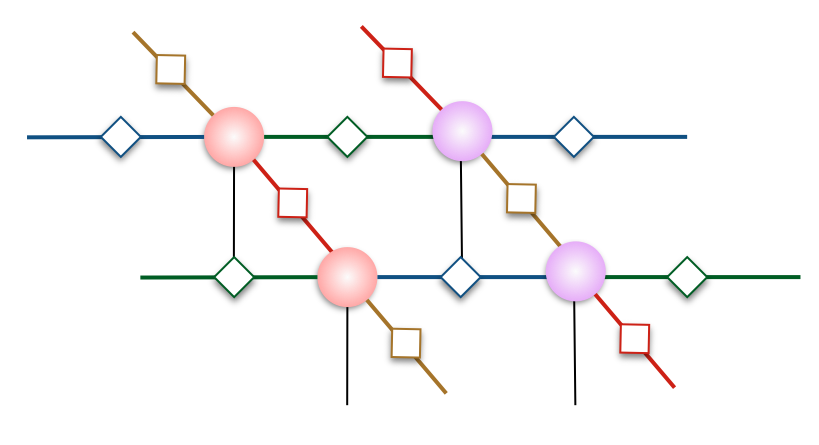
\includegraphics[width=0.6\textwidth]{figures/fig314.png}
	\caption[The tensor diagrams of 2-D lattice]{Four sites unit cell in iPEPS.}
	\label{fig314}
\end{figure}

After setting the form of iPEPS, we start to deal the question of updating states. The most intuitive scheme is to apply the scheme of \textit{Simple Update} which is shown in Fig.\ref{fig315}. The steps are similar to the iTEBD on 1-D systems. However, there are some differences. Firstly, the projected entangled pair states is a rank-5 tensor. Secondly, there are more entangled should be considered, due to increased neighbor sites.

More theoretical descriptions are written in [\ref{}][\ref{}]. Here, we explain the methods with TNs and some simple pseudocodes. The basic idea of \textit{2-D iTEBD} is to update the states from four directions by \textit{Simple Update}. The example starting from updating the green bond is shown in Fig.\ref{fig315} and Fig.\ref{fig316},

\begin{figure}[ht]
	\centering
	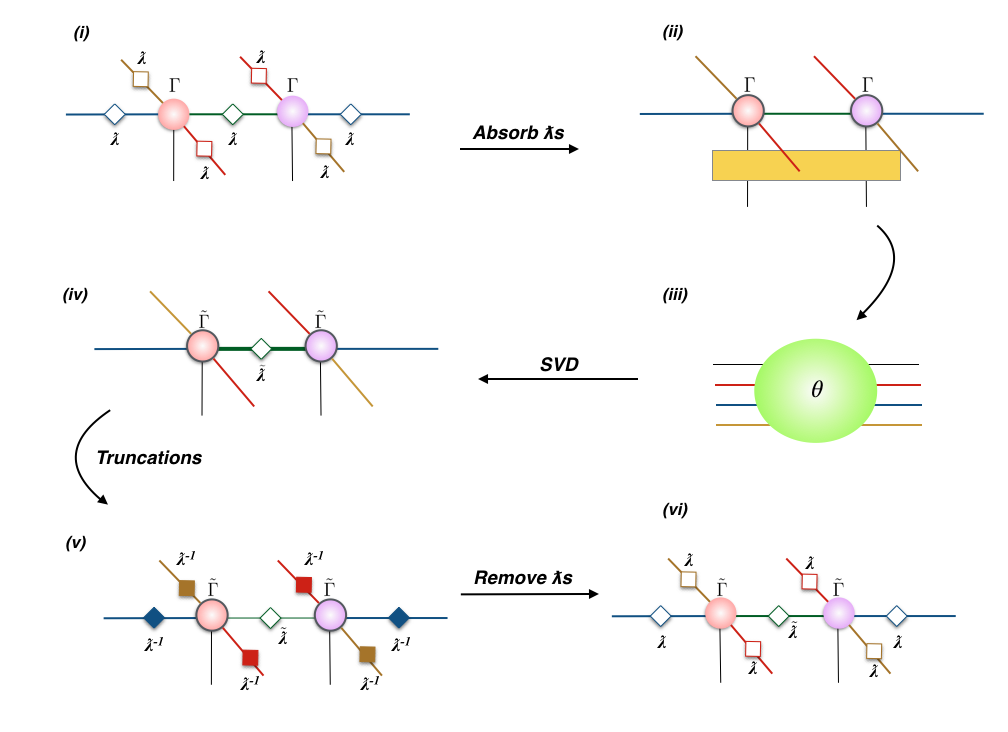
\includegraphics[width=1.00\textwidth]{figures/fig315.png}
	\caption[The tensor network diagrams of updating the green bond in iPEPS with 2D-iTEBD]{Absorb all $\lambda$ to $\Gamma$. (ii) Contract an evolution operator $e^{-\delta H}$ for evolving the system. (iii) Decompose the tensor $\theta$ by SVD. (iv) Truncate and Update the states and $\lambda$ on the green bond.(v) Remove $\lambda$ for obtaining the states. (iv) Obtain a original form of iPEPS. Repeat all the step to update the other bonds until the ground state energy convergence}
	\label{fig315}
\end{figure}

It's the same as one dimensional case, The first step is to absorb all $\lambda$ around the sites. The tensor with gray bold means the state have absorbed all entanglements. Secondly, contract the gate, $e^{-\delta H}$, for getting the tensor $\theta$. Thirdly, apply singular value decomposition to update states and the entanglement on the green bond. After decomposing $\theta$, we found that the dimension of the green bond increase to $dD^4$. Therefor, truncation plays a significant roles for keeping the dimension in the algorithm. In the end of the updating processes, multiply pseudo inverse of all $\lambda$ to the tensors for reducing to original form. 

	\begin{figure}[ht]
	\centering
	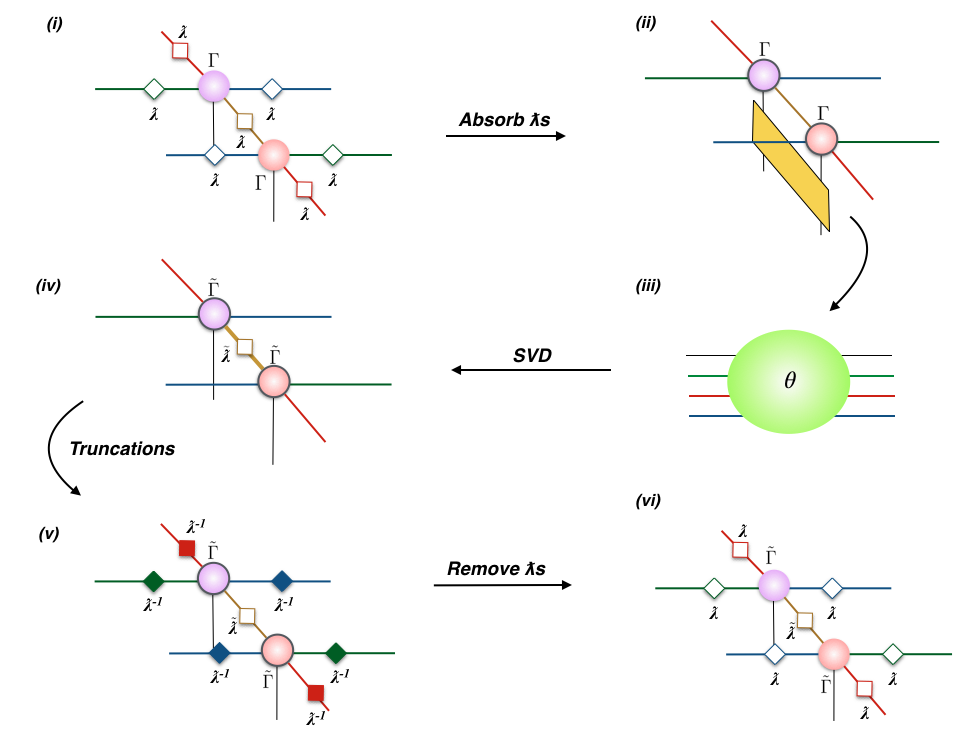
\includegraphics[width=1.00\textwidth]{figures/fig316.png}
	\caption[The tensor network diagrams of updating the yellow bond in iPEPS with 2D-iTEBD]{Update the yellow bond and the steps are similar to Fig.\ref{fig315}}
	\label{fig316}
	\end{figure}

	For easily to imagine how to updating the others directions. The updating steps of yellow bond are shown In Fig.\ref{fig316}.

%\begin{algorithm}
%	\caption{My algorithm}\label{euclid}
%	\begin{algorithmic}[1]
%		\Procedure{MyProcedure}{}
%		\State $\textit{stringlen} \gets \text{length of }\textit{string}$
%		\State $i \gets \textit{patlen}$
%		\BState \emph{top}:
%		\If {$i > \textit{stringlen}$} \Return false
%		\EndIf
%		\State $j \gets \textit{patlen}$
%		\BState \emph{loop}:
%		\If {$\textit{string}(i) = \textit{path}(j)$}
%		\State $j \gets j-1$.
%		\State $i \gets i-1$.
%		\State \textbf{goto} \emph{loop}.
%		\State \textbf{close};
%		\EndIf
%		\State $i \gets i+\max(\textit{delta}_1(\textit{string}(i)),\textit{delta}_2(j))$.
%		\State \textbf{goto} \emph{top}.
%		\EndProcedure
%	\end{algorithmic}
%\end{algorithm}


\section{Ameliorate two-dimensional iTEBD}
\label{2dhastin}

This method which make the algorithm more stable was published by \textit{M. B. Hastings}. Although \textit{Simple Update} shown in section.\ref{2ditebd} can obtain pretty good states, it's not stable and efficient enough. The reason is that too many multiplications of pseudo inverse $\lambda$ at the step Fig.\ref{fig315}(v). In numerical methods, it's hard to deal the problem of dividing the value which is equal or approach to zero. On the other words, the more inverse operations, the more the probability of bring about divergence or destroying algorithms.

For reducing the risk of breaking algorithms. Firstly, declare the states $\Gamma$ which include two entanglements among them. For instance, In Fig.\ref{fig317}(i), the red tensor is considered as multiplication of $A$ and the $\lambda$ on the yellow. The purple one is multiplication of $B$ and remained $\lambda$. Secondly, in Fig.\ref{fig317}(ii), because the entanglements on red and blue bonds are included in tensor $B$, we just need absorb the yellow one and contract the evolution operation for obtaining tensor $C$. Thirdly, we contract the red and blue $\lambda$ to the red and blue bonds which belong to the original tensor $A$ in tensor $C$ for getting $\theta$. Fourthly, getting the $\tilde{B}$ from decomposing and truncating $\theta$. Owing to avoid multiplying inverse matrices, we get $\tilde{A}$ by contracting tensor $C$ and $\tilde{B}$ and multiply an inverse $\lambda$ of yellow bond for removing the entanglement and reducing to original form.

	\begin{figure}[ht]
	\centering
	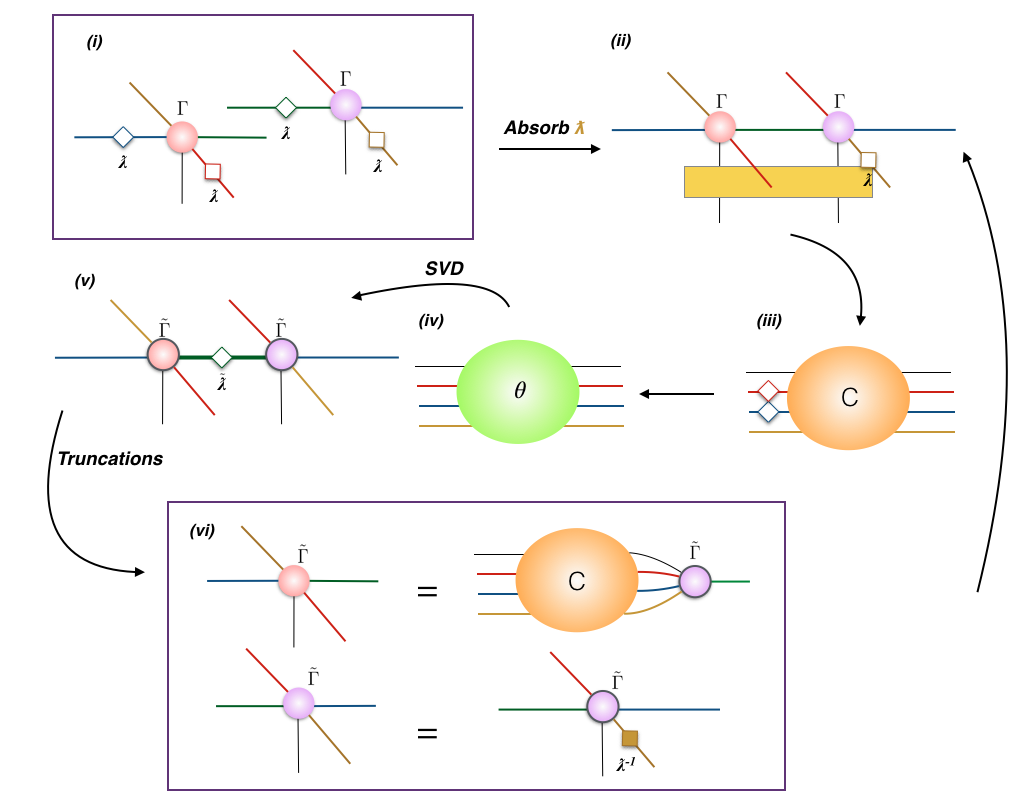
\includegraphics[width=1.00\textwidth]{figures/fig317.png}
	\caption[The tensor network diagrams for the 2-D iTEBD with QR decomposition]{The tensor network diagrams for the ameliorated 2-D iTEBD.}
	\label{fig317}
	\end{figure}

	Finally, repeat all the processes shown in Fig.\ref{fig317} to update different bonds until the convergence of the ground state energy.

\section{Optimizations}
\label{2dopt}

\subsection{Initialization}
\label{2doptInit}
Intuitively, the initialization of states should not affect the result. However, it's a serious misunderstanding. Actually, stating from a awful initial sates may break the algorithms or hardly converge.

From the viewpoint of physics, translational invariance is one of essential properties in many-body system, So we can assume that the group state on two sites should be similar. For instance, if the TN diagram of the states is shown as Fig \ref{fig321}(i), Fig \ref{fig321}(ii) might be the better way to initialize the states.

\begin{figure}[ht]
	\centering
	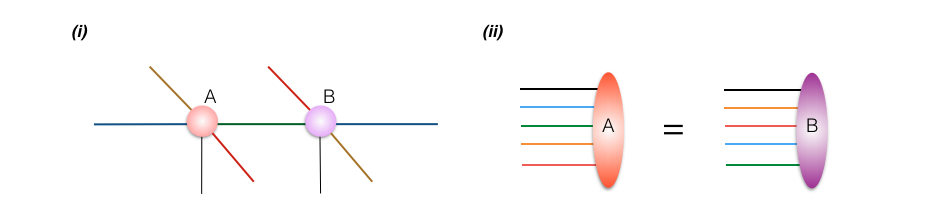
\includegraphics[width=1.00\textwidth]{figures/fig321.png}
	\caption[The diagrams of initializing projected entangled pair states]{(i) The structure of PEPS, (ii) The initialization of states}
	\label{fig321}
\end{figure}

\subsection{Truncattion Error}

\subsection{QR decomposition}

Though the strategy described in previous sections improve the stability, it's not efficient enough. The reason why is that the dimension of tensor $\theta$, in Fig.\ref{fig315}(iii) and Fig.\ref{fig317}(iii), is proportional to $d^2D^6$. In addition to that, the time complexity of singular value decomposition is proportional to $O(NM^2)$. In conclusion, the steps, in Fig.\ref{fig315}(iii) and Fig.\ref{fig317}(iii), are expensive, it is necessary to reduce the dimension of tensor $\theta$. 
\label{2doptQR} \begin{figure}[H] \centering 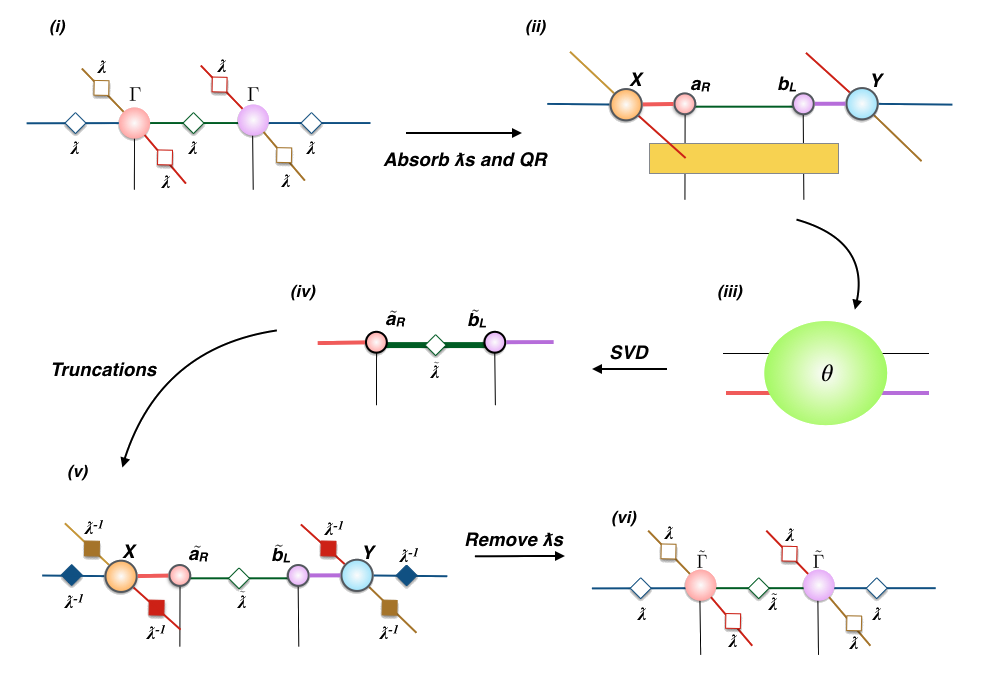
\includegraphics[width=0.80\textwidth]{figures/fig318.png} \caption[The tensor network diagrams for the ameliorated 2-D iTEBD with QR decompositiont]{The tensor network diagrams for the ameliorated 2-D iTEBD.} \label{fig318} \end{figure} To achieve the goal, the projected pair state must be decomposed by QR decomposition. The processes making \textit{Simple Update} more efficient is illustrated in Fig \ref{fig318}.  Most of the steps shown in Fig \ref{fig318} are like in Fig \ref{fig315}. The only difference is that after absorbing all the $\lambda$, we decompose the state to an orthogonal matrix and an upper triangular matrix by QR. For instance, in Fig \ref{fig318} (ii), the state $A$ is decomposed to an orthogonal matrix X and upper triangular matrix $a_R$. Due to the columns of $X$ are orthonormal, $XX^{\dagger}$ is equal to $I$. In the other word, the tensor $X$ can be ignored and we just need consider the tensor $a_R$ by QR. Similarity, the state $B$ can be decomposed to a lower triangular $b_L$ and an orthogonal matrix $Y$ by LQ which is equivalence to operate QR decomposition after transpose the matrix. Next, (iii) we can obtain the tensor $\theta$ whose dimension is $d^2D$ from $a_R$, $b_L$ and an evolution operator.

\begin{figure}[ht]
	\centering
	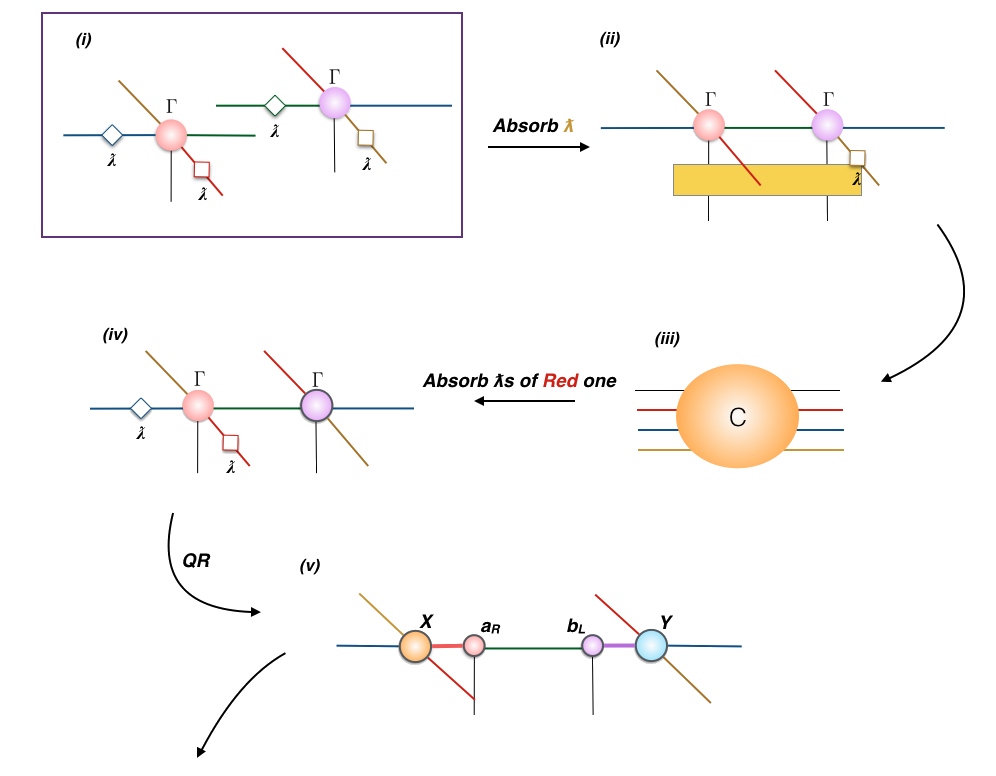
\includegraphics[width=0.90\textwidth]{figures/fig319.png}
	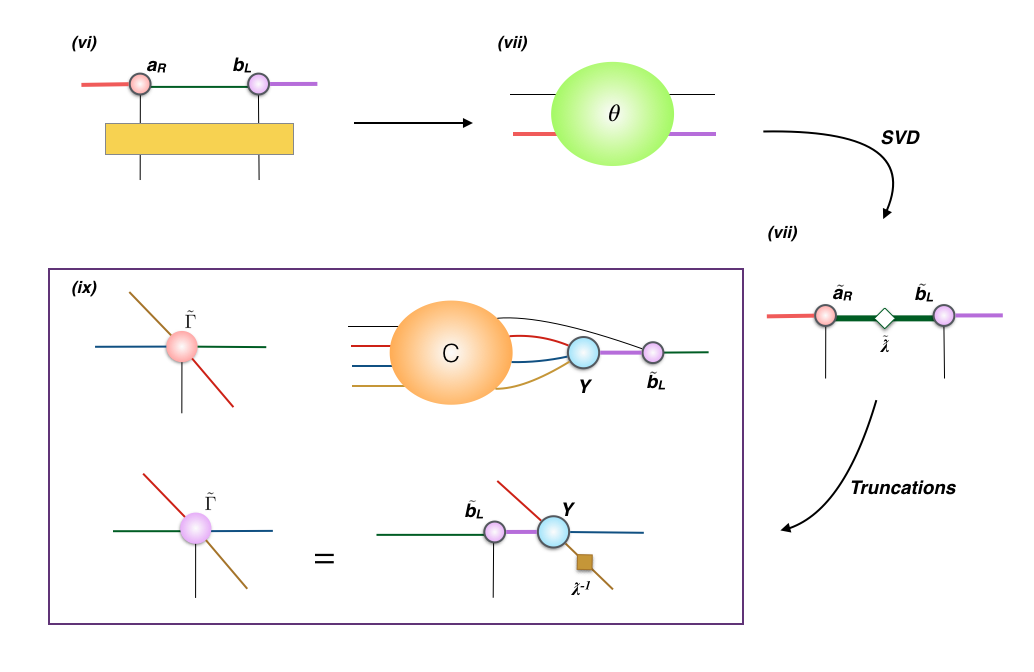
\includegraphics[width=0.90\textwidth]{figures/fig320.png}
	\caption[The tensor network diagrams for the ameliorated 2-D iTEBD with QR decompositiont]{The tensor network diagrams for the ameliorated 2-D iTEBD.}
	\label{fig319}
\end{figure}

The strategy to accelerate \textit{Ameliorate Simple Update} is shown in the Fig \ref{fig319} and its main idea is also to reduce the dimension of $\theta$.

\section{Comparison}

So far, we have benchmarked the improved iTEBD. 

\label{Comparison}
\subsection{Different Initializations}

\begin{figure}[ht]
	\centering
	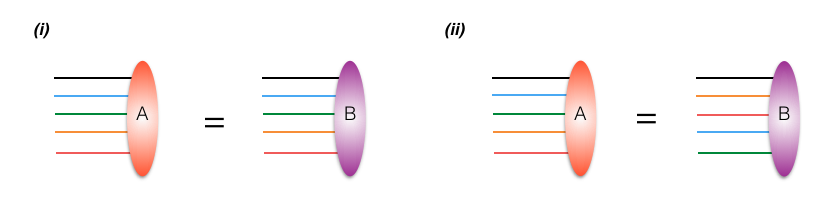
\includegraphics[width=1.00\textwidth]{figures/fig322.png}
	\caption[Different methods to initialize the states]{(i) Type 1, (ii) Type 2}
	\label{fig322}
\end{figure}

See Fig \ref{fig323}, the both cases are 

\begin{figure}[ht]
	\centering
	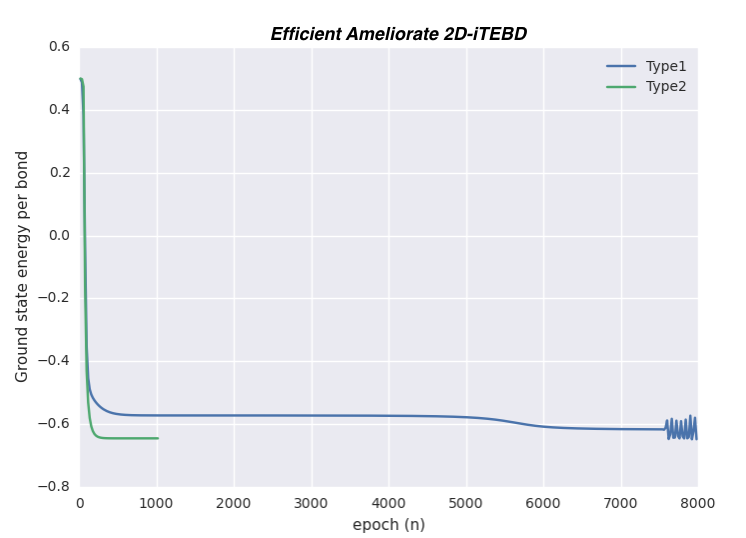
\includegraphics[width=0.75\textwidth]{figures/fig323.png}
	\caption[Comparison the results of Heisenberg model on square lattice which are obtaining from different initial states.]{The Blue line represents updating tensors from the initial state shown in Fig \ref{fig322} (i) and the green one represents updating from Fig \ref{fig322} (ii)}
	\label{fig323}
\end{figure}

\begin{figure}[ht]
	\centering
	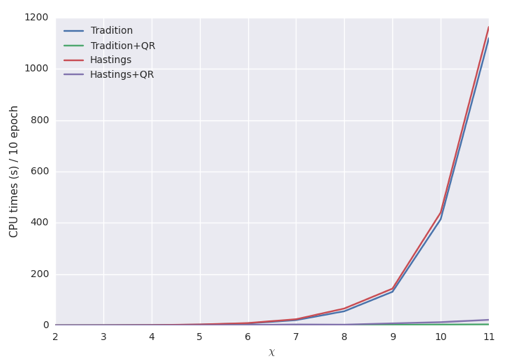
\includegraphics[width=0.75\textwidth]{figures/fig324.png}
	\caption[tmp]{}
	\label{fig324}
\end{figure}

\begin{figure}[ht]
	\centering
	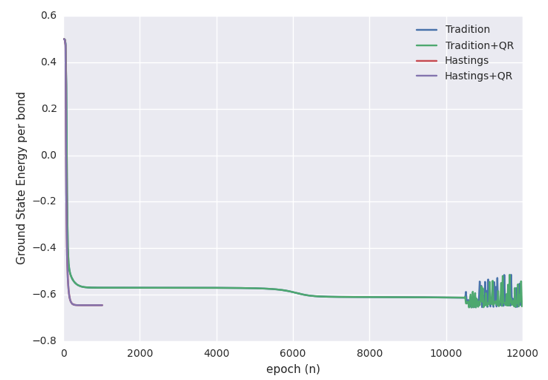
\includegraphics[width=0.75\textwidth]{figures/fig325.png}
	\caption[tmp]{}
	\label{fig325}
\end{figure}

\begin{figure}[ht]
	\centering
	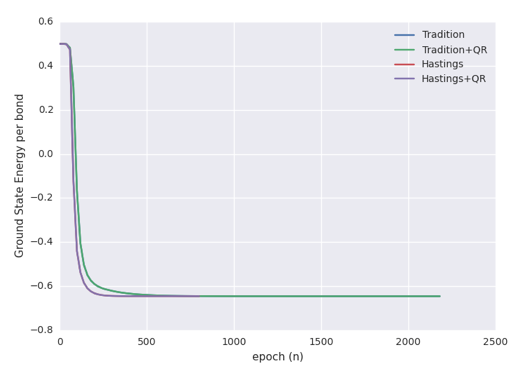
\includegraphics[width=0.75\textwidth]{figures/fig326.png}
	\caption[tmp]{}
	\label{fig326}
\end{figure}

\begin{figure}[ht]
	\centering
	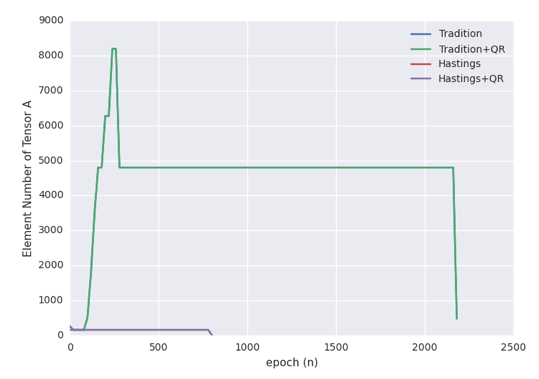
\includegraphics[width=0.75\textwidth]{figures/fig327.png}
	\caption[tmp]{}
	\label{fig327}
\end{figure}

%!TEX root = thesis.tex
\chapter{Infinite Projected Entangled Simplex State}
\label{chapter:ipess}

\section{Infinite Kagome Lattice}
\subsection{3-PESS}
\label{3pess}

\subsection{5-PESS}
\label{5pess}

\section{Infinite Square Lattice}
\subsection{4-PESS (local tensors are rank-2)}
\label{4pess2b}
\subsection{4-PESS (local tensors are rank-4)}
\label{4pess4b}


%!TEX root = thesis.tex
\chapter{Corner Transfer Matrix}
\label{chapter:ctm}
The \textit{cerner transfer matrix renormalization group} (CTMRG) \cite{doi:10.1143/JPSJ.65.891} \cite{PhysRevB.80.094403} \cite{PhysRevB.84.041108} is an algorithm to numerically compute the \textit{effective environments} which is an approximation of the environment of systems. For example, if the infinite PEPS is composed by a single tensor $A^{h}_{uldr}$ repeatedly, where $h$ express a physical basis of  $\mathbb{V}$ with dimension $d$, and $u,l,d,r$ are virtual bonds with dimension $D$, see Fig.~\ref{fig501}(a). Then we can represent the scale norm $\Braket{\psi|\psi}$ by a simple two dimensional tensor network $\varepsilon$ which is characterized by reduced tensors $a$, shown in Fig.~\ref{fig501}(b). The reduced tensor $a$ is defined as eq.\ref{reduce_a}, 
\begin{align}
	\label{reduce_a}
	a \equiv \sum_{h=1}^{d} A_{h} \otimes A^{*}_{h}
\end{align}
The environment $\varepsilon^{[\vec{r}]}$ of the site $\vec{r}$ could be described by the reduced tensors in the gray rectangles in Fig.\ref{fig501}(c) and the \textit{effective environments} $G^{[\vec{r}]}$ shown in Fig.~\ref{fig501}(d) is target of the CTMRG. 

In the following subsections, we will show more details of implementation of CTM and compare some features between obtaining the states from iPEPE and PESS.

\begin{figure}[ht]
	\centering
	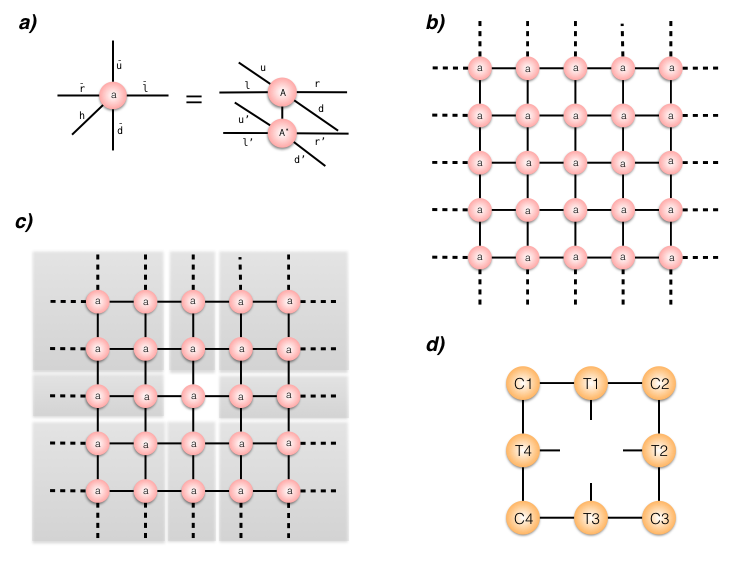
\includegraphics[width=0.75\textwidth]{figures/fig501.png}
	\caption[The tensor diagrams of the corner transfer matrix with the one-site unit cell.]{The tensor diagrams of corner transfer matrix. (a) The reduced tensor $a$ is obtained from the iPEPS state $A$, where $a \equiv \sum_{h=1}^{d} A_{h} \otimes A^{*}_{h}$. (b) An infinite two-dimensional tensor network $\varepsilon$ . (c) The environment $\varepsilon^{[\vec{r}]}$of the site $\vec{r}$. (d) The effective environment $G^{[\vec{r}]}$.}
	\label{fig501}
\end{figure}

\section{Obtain States from PEPS}
\label{2ditebdctm}
In chapter.\ref{chapter:2ditebd}, we have discussed about obtaining the infinite PEPS state $\Ket{\psi}$ of an infinite 2D square lattice by imaginary time evolution and known that the infinite PEPS could be characterized by two tensors $A^h_{uldr}$ and $B^h_{drul}$ repeatedly (Fig.~\ref{fig511}(a)). The scalar norm of the iPEPS $\Braket{\psi|\psi}$ is composed by reduced tensors $a_{\bar{u}\bar{l}\bar{d}\bar{r}}$ and $b_{\bar{d}\bar{r}\bar{u}\bar{l}}$(Fig.~\ref{fig511}(b)), where
\begin{align}
	\label{reduce_a}
	\bar{a} \equiv \sum_{h=1}^{d} A_{h} \otimes A^{*}_{h} \\
	\label{reduce_b}
	\bar{b} \equiv \sum_{h=1}^{d} B_{h} \otimes B^{*}_{h}
\end{align}

Then, we can consider the environment $\varepsilon^{\left[\vec{r_1},\vec{r_2},\vec{r_3},\vec{r_4}\right]}$ of a four-site structure (Fig.~\ref{fig511}(c)), and try to approximate it with effective environment $G^{\left[\vec{r_1},\vec{r_2},\vec{r_3},\vec{r_4}\right]}$ (Fig.~\ref{fig511}(d)), which consists of $C_1, T_{a1}, T_{b1},C_2, T_{a2}, T_{b2},C_3, T_{a3}, T_{b3},C_4, T_{a4}, T_{b4},$

\begin{figure}[ht]
	\centering
	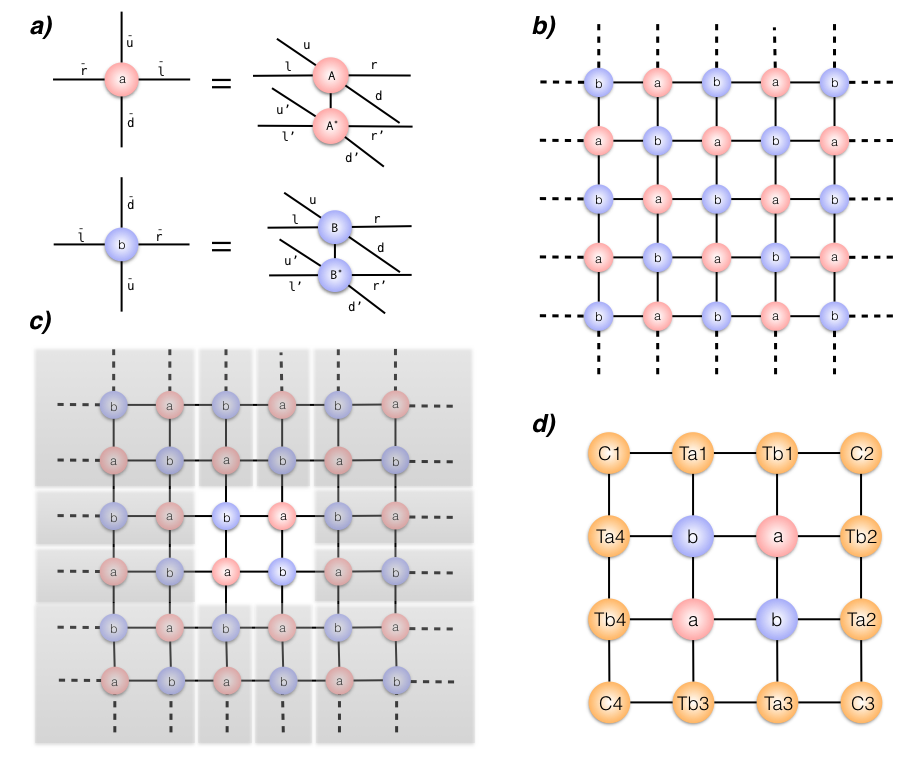
\includegraphics[width=0.75\textwidth]{figures/fig511.png}
	\caption[The tensor diagrams of the corner transfer matrix with the four-site unit cell.]{The tensor diagrams of the corner transfer matrix with the four-site unit cell.(a) The reduced tensor $a$ and $b$ are obtained from the iPEPS state $A$ and $B$, where $a \equiv \sum_{h=1}^{d} A_{h} \otimes A^{*}_{h}$ and $b \equiv \sum_{h=1}^{d} B_{h} \otimes B^{*}_{h}$. (b) An infinite two-dimensional tensor network $\varepsilon$. (c) The environment of the four-site unit cell. (d) The effective environment $G^{\left[\vec{r_1},\vec{r_2},\vec{r_3},\vec{r_4}\right]} = \{ C_1, T_{a1}, T_{b1},C_2, T_{a2}, T_{b2},C_3, T_{a3}, T_{b3},C_4, T_{a4}, T_{b4}\}$.}
	\label{fig511}
\end{figure}

For the approximation of environment, the directional variant of the CTMRG was developed. According to \textit{directional coarse-graining moves}, the effective environment could be updated from four different moves , left, right, up and down and iterated until the environments converges. 

For instance, the procedures to the left move, shown in the Fig.~\ref{fig512} which is derived by Roman and Vidal, is made up of four major steps,
\begin{enumerate}
	\item Insertion: Insert two new columns which consist of \{ $T_{a1},b,a,T_{b3}$ \} and \{ $T_{b1},a,b,T_{a3}$ \} as in Fig.~\ref{fig512}(b).
	\item Absorption: In order to obtaining two new corner matrices $\tilde{C_1}$ and $\tilde{C_4}$, and two new transfer matrices $\tilde{T_{b4}}$ and $\tilde{T_{a4}}$, we contract tensors $C_1$ and $T_{b1}$, tensors $C_3$ and $T_{a3}$, tensors $T_{a4}$ and $b$, and tensors $T_{b4}$ and $a$. Then, contract tensors $\tilde{C_1}$ and $\tilde{T_{b4}}$, and tensors $\tilde{C_4}$ and $\tilde{T_{a4}}$, obtaining $\tilde{Q_1}$ and $\tilde{Q_4}$ which play significant rules for calculating isometries between $\tilde{T_{b4}}$ and $\tilde{T_{a4}}$ as in Fig.~\ref{fig512}(c).
	\item Renormalization: Truncate the vertical virtual bonds of $\widetilde{C_1}$, $\widetilde{T_{b4}}$, $\widetilde{T_{a4}}$, and $\widetilde{C_4}$ by contracting the isometries $Z$ and $W$, where
\begin{align}
	\label{isometry}
	&Z^{\dagger}Z = I \\
	&W^{\dagger}W = I
\end{align}
and the renormalization of the left CTM, yield as
\begin{align}
	\label{renormalize}
	&C^{\prime}_1 = Z^{\dagger} \tilde{C_1} \\
	&T_{b4}^{\prime} = Z\tilde{T_{b4}}W^{\dagger} \\
	&T_{a4}^{\prime} = W\tilde{T_{b4}}Z^{\dagger} \\
	&C^{\prime}_4 = Z\widetilde{C_4}
\end{align}
See the Fig.~\ref{fig512}(d) and \ref{fig512}(f).
	\item Truncation: To determinate the isometries Z and W in the \textit{renormalization} steps is the most significant part. In this case, we use the eigenvalue decomposition of 
		\begin{align}
			\label{eigh_ctm}
			&\tilde{C_1}\tilde{C^{\dagger}_1}+\tilde{C_4}\tilde{C^{\dagger}_4}= \tilde{Z} D_z \tilde{Z^{\dagger}}\\
			&\tilde{Q_1}\tilde{Q^{\dagger}_1}+\tilde{Q_4}\tilde{Q^{\dagger}_4}= \tilde{W} D_w \tilde{W^{\dagger}}
		\end{align}
		shown in Fig.~\ref{fig512}(e). It's not hard to find that the 
		the dimension of bonds of $D_z$ and $D_w$ increase to $\chi^2$. For that reason, we have to truncate $\tilde{Z}$ and $\tilde{W}$ to isometries $Z$ and $W$ which are equivalent to keeping the columns of $\tilde{Z}$ and $\tilde{W}$ corresponding to $\chi$ largest eigenvalues of $D_z$ and $D_w$.
\end{enumerate}

Now, we need repeat the procedures in Fig.~\ref{fig512}(b)-(d) again for absorbing the other inserted column in Fig.~\ref{fig512}(d) and obtain a new effective environment $G^{\prime \left[\vec{r_1},\vec{r_2},\vec{r_3},\vec{r_4}\right]}$ for the four-site unit cell. By composing four variant moves of the CTM we build an epoch of CTMRG. 

\begin{figure}[ht]
	\centering
	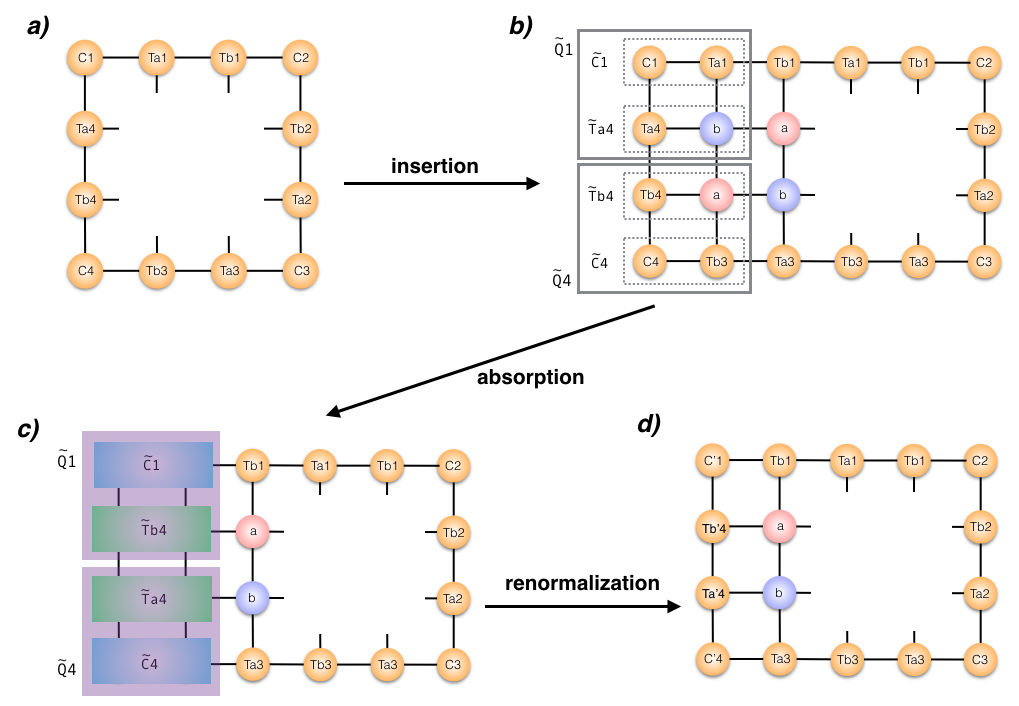
\includegraphics[width=0.80\textwidth]{figures/fig512.png}
	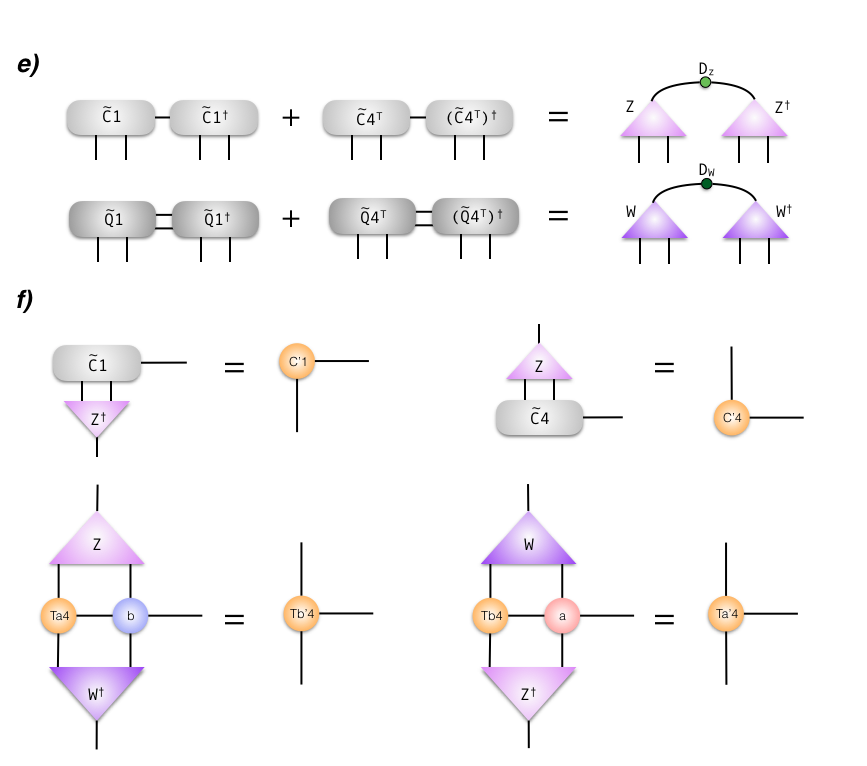
\includegraphics[width=0.80\textwidth]{figures/fig513.png}
	\caption[The procedures of the corner transfer matrix.]{The procedures of the corner transfer matrix. The more discussions are derived in the paragraph}
	\label{fig512}
\end{figure}

\section{Obtain States from PESS}
\label{pessctm}
In this section, we apply the CTM to approximate the effective environment of 4-PESS structure. Firstly, we must transform it to iPEPS structure which is suit for the form of CTM. As shown in Fig.~\ref{fig521}, the projection tensors, $U^{[0]}$, $U^{[1]}$, $U^{[2]}$ and $U^{[3]}$, and the entangled simplex tensors, $S^{[\alpha]}$ and $S^{[\beta]}$ are obtained from 4-PESS ansatz. To map these states to PEPS-like structure, we group the tensors, $S^{[\alpha]}$, $U^{[0]}$ and $U^{[1]}$, in red rectangles into the tensor $A$, 
\begin{align}
	A^{\sigma_i \sigma_j}_{i^{\prime}j^{\prime}kl} = \sum_{ij}{U^{[0]}_{ ii^{\prime},\sigma_i} S^{[\alpha]}_{ijkl} U^{[1]}_{ jj^{\prime},\sigma_j}}
\end{align}
and group, $S^{[\beta]}$, $U^{[2]}$ and $U^{[3]}$, in blue rectangles into the tensor $B$
\begin{align}
	B^{\sigma_k \sigma_l}_{i^{\prime}j^{\prime}kl} = \sum_{k^{\prime}l^{\prime}}{U^{[2]}_{ kk^{\prime},\sigma_i} S^{[\beta]}_{i^{\prime}j^{\prime}k^{\prime}l^{\prime}} U^{[3]}_{ ll^{\prime},\sigma_j}}
\end{align}
, whee the ranks of tensor $A$ and $B$ are six and there are two physical bonds contained in each of them. Hence, after combined the physical bonds in tensors $A$ and $B$, the iPEPS structure will be obtained,
\begin{align}
	A^{\sigma_i \sigma_j}_{i^{\prime}j^{\prime}kl} \rightarrow  A^{\sigma_A}_{i^{\prime}j^{\prime}kl} \\
	B^{\sigma_k \sigma_l}_{i^{\prime}j^{\prime}kl} \rightarrow  B^{\sigma_B}_{i^{\prime}j^{\prime}kl}
\end{align}
Next, in order to make the structure more balance, the entanglement should be well-distributed between each sites, 
\begin{align}
	\widetilde{A} = \sum_{i^{\prime}j^{\prime}kl}{\lambda^{[\beta]^{\frac{1}{2}}}_{i^{\prime}} \lambda^{[\beta]^{\frac{1}{2}}}_{j^{\prime}} A^{\sigma_A}_{i^{\prime}j^{\prime}kl}\lambda^{[\alpha]-\frac{1}{2}}_{l} \lambda^{[\alpha]^{-\frac{1}{2}}}_{k}}\\
	\widetilde{B} = \sum_{i^{\prime}j^{\prime}kl}{\lambda^{[\alpha]^{\frac{1}{2}}}_{k} \lambda^{[\alpha]^{\frac{1}{2}}}_{l} B^{\sigma_B}_{i^{\prime}j^{\prime}kl} \lambda^{[\beta]^{-\frac{1}{2}}}_{i} \lambda^{[\beta]^{-\frac{1}{2}}}_{j^{\prime}}}
\end{align}
and substitute $\widetilde{A}$ and $\widetilde{B}$ into Eq. \ref{reduce_a} and Eq. \ref{reduce_b} to obtain reduced tensors $a$ and $b$. In the end, we apply these two reduced tensor to build the form of CTM and follow the procedures shown in Fig.~\ref{fig512} to simulate the effective environment tensors.

\begin{figure}[ht]
	\centering
	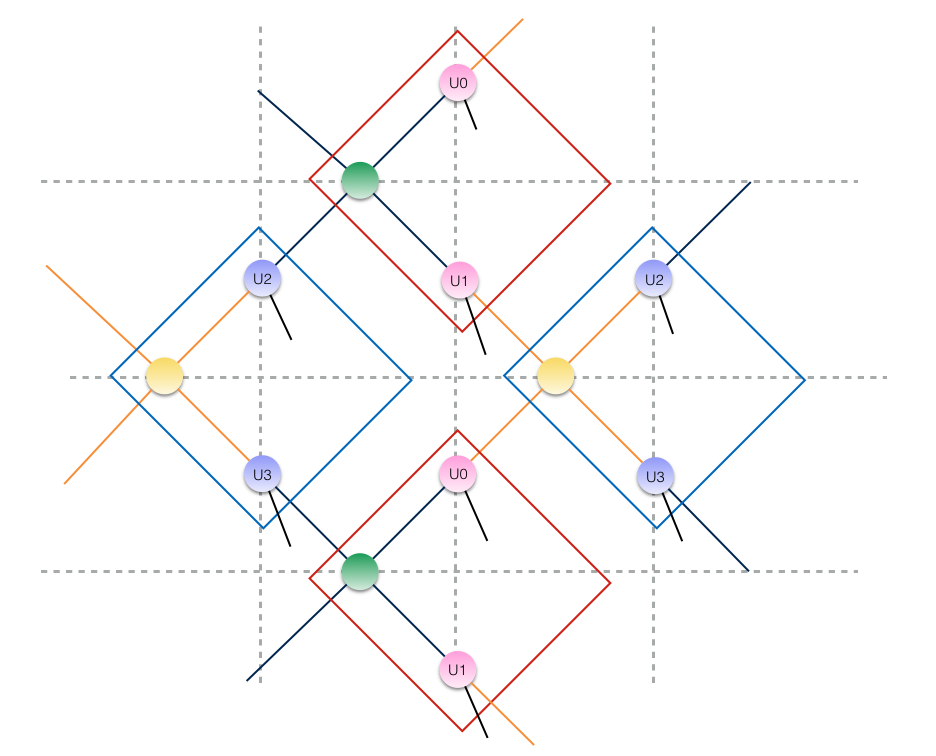
\includegraphics[width=0.70\textwidth]{figures/fig521.png}
	\caption[The tensor diagram of obtaining the reduce tensors from 4-PESS structure.]{The tensor diagram of obtaining the reduce tensors from 4-PESS structure. The reduce tensor $a$ and $b$ are composed by the tensors in the red and blue rectangles}
	\label{fig521}
\end{figure}

\section{Comparison}

To compare the performance of the approximations, we have applied 2D-iTEBD and PESS to approach the ground state of the spin-1/2 quantum transverse Ising model, 
\begin{align}
	H = -\sum_{<\vec{r},\vec{r}^{\prime}>}{\sigma_z^{[ \vec{r}^{} ]} \sigma_z^{[ \vec{r}^{\prime} ]}} - \lambda \sum_{\vec{r}}{\sigma_x^{[ \vec{r} ]}}
\end{align}
, and use directional CTM to obtain the effective environment at each sides. See Fig.~\ref{fig522}, the order-parameter $m_z \equiv  \Bra{\Psi} \sigma_z \Ket{\Psi}$ as a function of the external magnetic field $\lambda$. We find that when measuring the local observable with directional CTM, the better ground states are obtained. However, it have no improvement when approaching to near-critical point. The possible reason is that 
the original states computed by iPEPS approximation is not accuracy sufficiently. Next, turn to the cases which states are obtained from 4-PESS algorithm.When $D=2$ and $\chi = 20$, we find that it is hard to converge near the critical point because the virtual bonds dimension too small to describe the systems. After increasing the virtual dimension, we notice that it converge to $\lambda_c \approx 3.220$. In Sec.~\ref{chapter:ipess}, we have shown that the ground states obtained by 4-PESS has more accuracy. Hence, it is not astonish that the result compute with 4-PESS+CTM is better than 2D-iTEBD+CTM. However, it still can not compare with  the quantum Monte Carlo estimation which is $\lambda^{MC}_c \approx 3.044$ \cite{PhysRevE.66.066110}.

\begin{figure}[H]
	\centering
	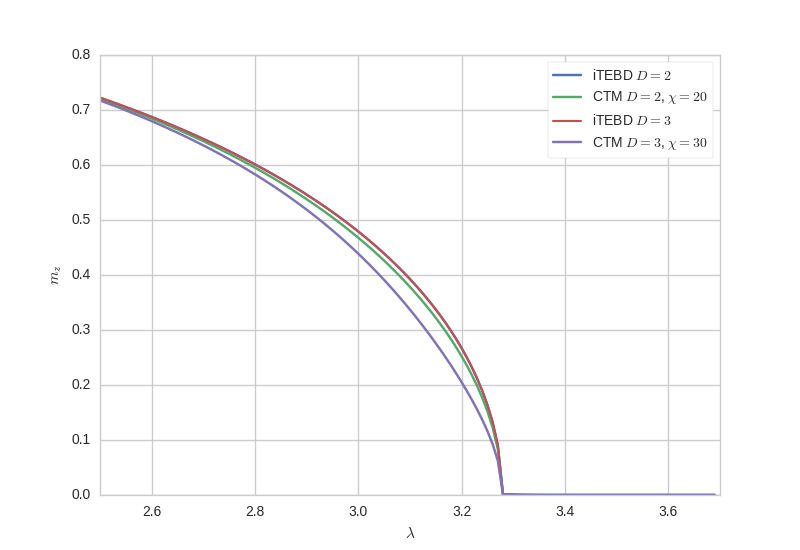
\includegraphics[width=0.75\textwidth]{figures/ctm_itebd.png}
	\caption[Compare the order-parameter $m_z$ of the transfer Ising model on square lattice between 2D-iTEBD and 2D-iTEBD+CTM.]{Compare the order-parameter $m_z$ of the transfer Ising model on square lattice between 2D-iTEBD and 2D-iTEBD+CTM, where the order-parameter $m_z$ as a function of the external field $\lambda$}
	\label{fig522}
\end{figure}

\begin{figure}[H]
	\centering
	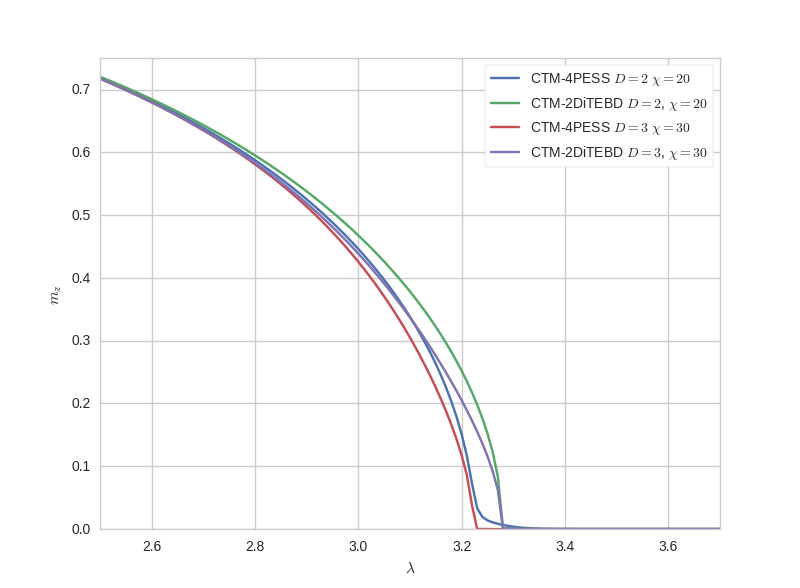
\includegraphics[width=0.75\textwidth]{figures/ctm_pess.png}
	\caption[Compare the order-parameter $m_z$ of the transfer Ising model on square lattice between 2D-iTEBD+CTM and 4-PESS+CTM.]{Compare the order-parameter $m_z$ of the transfer Ising model on square lattice between 2D-iTEBD+CTM and 4-PESS+CTM, where the order-parameter $m_z$ as a function of the external field $\lambda$}
	\label{fig523}
\end{figure}



%!TEX root = thesis.tex
\chapter{Full Update}
\label{chapter:fupdate}

\section{Properties}
\label{fupdateproperties}

\section{Optimization}
\subsection{Initialization}
\label{optfupdateint}

\subsection{Reduce the dimensions of virtual bonds with QR decomposition}
\label{optfupdateqr}

\subsection{Gauge fixing}
\label{optfupdatefix}

\section{Fast Full Update}
\label{ffupdate}


\appendix


\addcontentsline{toc}{chapter}{\bibname}
%\bibliographystyle{unsrtnat}
\bibliographystyle{apsrev4-1}
%\bibliographystyle{plainnat}
%\bibliographystyle{apalike}

% Your bibliography goes here
\bibliography{thesis}
%\makespine
\end{document}
